\documentclass{article}
\usepackage[utf8]{inputenc}
\usepackage{amsmath}
\everymath{\displaystyle}
\usepackage{biblatex}
\addbibresource{referencias.bib}

\usepackage{hyperref}
\usepackage[spanish, es-tabla]{babel}

\usepackage{authblk}
\renewcommand\Authand{ y }
\renewcommand\Authands{, y }
\renewcommand*{\Authfont}{\bfseries}
%% Page settings
\usepackage[a4paper, margin=1in]{geometry}
\usepackage{graphicx}
\usepackage{multirow}
\usepackage{float}
\usepackage{caption}
\usepackage{subcaption}
\usepackage{lipsum}
\usepackage{wrapfig}
\usepackage{booktabs}
\usepackage{siunitx}
\DeclareSIUnit{\calorie}{cal}
\usepackage{amsmath}
\usepackage{multicol}

\usepackage[table]{xcolor}
\renewcommand{\d}{\text d}
\newcommand{\dd}[2]{\frac{\d #1}{\d #2}}
\newcommand{\ddp}[2]{\frac{\partial #1}{\partial #2}}

\newcommand{\myfigure}[4][0.65]{%
    \vspace{1em}
    \noindent\begin{minipage}{\linewidth}%
        \makebox[\linewidth]{%   For centring figures
            \includegraphics[width=#1\linewidth]{#2}}
        \captionof{figure}{#3}
        \label{#4}
    \end{minipage} 
    \vspace{0.5em}}

\usepackage{amsfonts}
\newcommand{\overbar}[1]{\mkern 1.5mu\overline{\mkern-1.5mu#1\mkern-1.5mu}\mkern 1.5mu}

\title{\vspace{-15mm}\fontsize{24pt}{10pt}\selectfont\textbf{Máquinas Térmicas}} % Article title 

\author{Andrés David Rojas Lozano}
\author{Andrés Esteban Leal Buitrago}
\author{Gabriel Sandoval Velásquez}
 
\affil{Universidad Nacional de Colombia}
\affil{\{
    \href{mailto:androjaslo@unal.edu.co}{androjaslo}, 
    \href{mailto:aelealb@unal.edu.co}{aelealb}, 
    \href{mailto:gfsandovalv@unal.edu.co}{gfsandovalv}
    \}@unal.edu.co}

\date{\today}

\begin{document}
\maketitle
%\begin{multicols}{2}
\begin{abstract}
    Se calcula la eficiencia $\eta$ y coeficiente de rendimieto $COP$ para la celda Peltier, usada como generador termoeléctrico y como refrigerador, respectivamente. 
\end{abstract}


\section{Introducción}
\subsection{Máquinas térmicas}
Una máquina térmica es un conjunto de elementos mecánicos que permiten intercambiar energía, la cual usando el primer principio de la termodinámica, toma calor de una fuente y logra convertir parte de ella en
trabajo, esto en un proceso cíclico.

La eficiencia de este sistema es definida a partir del trabajo(W) que realiza y el calor que recibe de la fuente($Q_H$), como:

\begin{equation}
    \eta = \frac{W}{Q_H}=\frac{P_W}{P_H}
\end{equation}
Donde $P_H=P_W+P_C$

\subsection{Principio cero de la termodinámica}

Este principio establece que dos o más cuerpos en contacto que se encuentran a distinta temperatura alcanzan, pasado un tiempo, a través de un intercambio de energía, el equilibrio térmico; este intercambio depende del tipo de trasformación que ha experimentado el sistema y a esta transferencia es a la que se le llama calor, entonces los cuerpos no almacenan calor sino energía interna. La expresión que relaciona la cantidad de calor $Q[J]$ que intercambia una cierta sustancia de masa $m[g]$ y calor específico $c_e[J/g°C]$ con la variación de temperatura $\Delta T[°C]$ que experimenta es:
\begin{equation}
    Q=mc_e\Delta T
\end{equation}

\subsection{Segundo principio de la termodinámica}
Este principio establece la irreversibilidad de los fenómenos físicos, especialmente durante el intercambio de calor. Es un principio de la evolución que fue enunciado por primera vez por Sadi Carnot en 1824. Después ha sido objeto de numerosas generalizaciones y formulaciones sucesivas por Clapeyron (1834), Clausiuos(1850), Lord Kelvin, Ludwig Boltzmann en 1873 y Max Planck.

Según Planck, es imposible construir un motor que, trabajando según un ciclo completo, no produzca otro efecto que elevar un peso y enfriar una fuente caliente.

\subsection{Ciclo de Carnot}
Este es un ciclo termodinámico que se produce una maquina cuando trabajo absorbiendo una cantidad de calor de una fuente de mayor temperatura cede calor a una de menor temperatura produciendo un trabajo. 

Este ciclo está conformado por 4 procesos, el primero es una expansión isoterma ( A $\rightarrow$ B), después una expansión adiabática (B $\rightarrow$ C), después una comprensión isoterma (C $\rightarrow$ D) y por ultimo una compresión adiabática ( D $\rightarrow$ A). La máxima eficiencia de este ciclo está dada por:
\begin{equation}
    \eta_{Carnot}=\frac{T_H-T_C}{T_H}
\end{equation}
La eficicencia para una máquina térmica real es menor que esta dadas las pérdidas por fricción, conducción, radiación y calentamiento.
\begin{figure}[H]
    \centering
    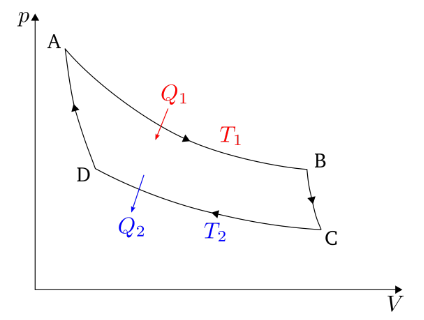
\includegraphics[scale=0.6]{img/carnot.png}
    \caption{Ciclo de Carnot en diagrama P y V}
    \label{fig:my_label}
\end{figure}

\subsection{Frigoríficos}
Un frigorífico es una máquina que funciona en sentido contrario a una maquina térmica, de tal forma que extrae calor de la fuente fría a la fuente caliente.

La eficiencia de esas máquinas se define de forma distinta las máquinas térmicas. Se define el coeficiente de rendimiento (COP por sus siglas en ingles), el cual es la razón entre el calor bombeado de la fuente fría y el trabajo requerido para realizarlo, entonces:
\begin{equation}
    k=COP=\frac{Q_c}{W}=\frac{P_c}{P_W}
\end{equation}
También podemos hablar de una eficiencia máxima o eficiencia de carnot para frigoríficos dada por:

\begin{equation}
    k_{Max}=\frac{T_C}{T_H-T_C}
\end{equation}

\subsection{Motor de Stirling}
Un motor Stirling es un motor térmico operando por compresión y expansión cíclica de aire u otro gas, llamado fluido de trabajo, a diferentes niveles de temperatura tales que se produce una conversión neta de energía calorífica a energía mecánica.
\begin{figure}[H]
    \centering
    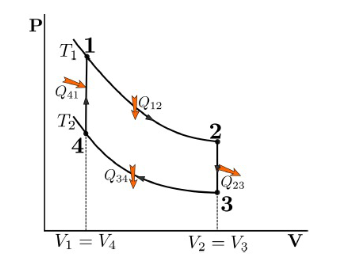
\includegraphics[scale=0.6]{img/stirling.png}
    \caption{Ciclo de un motor Stirling en diagrama P y V}
    \label{fig:my_label}
\end{figure}

\subsection{Módulo termoeléctrico}
Un modulo termoeléctrico es un dispositivo que basado en el efecto Seebeck, efecto Peltier y efecto Thomson crea un flujo térmico a través de la unión de dos materiales diferentes.

\begin{itemize}
    \item \textbf{Efecto Seebeck:}\\ cuando se forma un circuito
cerrado a partir de dos materiales distintos y se mantienen bajo las uniones una diferencia de temperatura, se produce una corriente electrica denominada termocorriente,la cual depende de la temperatura relativa entre los contactos y la naturaleza de los materiales. La diferencia de potencial a lo largo del circuito esta dada de la forma:
\begin{equation*}
    \Delta V = \oint_T^{T+\Delta T} (S_A-S_B)dT
\end{equation*}
Dónde S se define como el coeficiente de Seebeck, $S=-(\frac{dV}{dT})_T$
\item \textbf{Efecto Peltier:}\\ Este efecto realiza la acción inversa al efecto Seebeck. Consiste en la creación de una diferencia
térmica a partir de una diferencia de potencial eléctrico. Ocurre cuando una corriente pasa a través de dos metales diferentes o semiconductores (tipo-n y tipo-p) que están conectados entre sí
en dos soldaduras (uniones Peltier). La corriente produce una transferencia de calor desde una unión, que se enfría, hasta la otra, que se calienta.
\item \textbf{Efecto Thomson:}\\ El efecto Thomson fue predicho y luego observado experimentalmente por William Thomson (Lord Kelvin) en 1851. Describe el calentamiento o enfriamiento de un conductor portador de corriente con un gradiente de temperatura.

\end{itemize}
\section{Marco teórico}

\section{Descripción experimental}

\section{Resultados y análisis}

A continuación se muestran las potencias calculadas a partir de los datos experimentales para cada montaje. 
\subsection{Generador Termoeléctrico}

A partir de los datos medidos (temperatura y voltajes) se obtienen las potencias, aplicada $P_A$, de carga $P_L$ y disipada por la resistencia interna $P_{R_i}$. Además, se interpolan los valores de $P_{open}$ usando una regresión de los datos suministrados. Estos datos se tomaron usando una escala de temperatura con precisión de décimas de grado y un rango de diferencia de temperatura  $\Delta T = 0 - 40 \si{\celsius}$. Estos valores se muestran en la figura \ref{fig:gen_powers}. Se observa que los datos de $P_A$ tienen un comportamiento escalonado, esto debido a que al aplicar una diferencia de potencial a la resistencia de carga, se debía dejar transcurrir un tiempo hasta observar la temperatura máxima alcanzada por la resistencia de calentamiento, y en ese tiempo, por lo que se registraron varios datos para un mismo voltaje aplicado. De la gráfica \ref{fig:gen_powers} también se puede corroborar que los datos obtenidos para las demás potencias son menores a la potencia aplicada, corroborando que la energía útil en efecto es menor que la energía suministrada, en concordancia con la segunda ley.

\begin{figure}[ht]
    \centering
    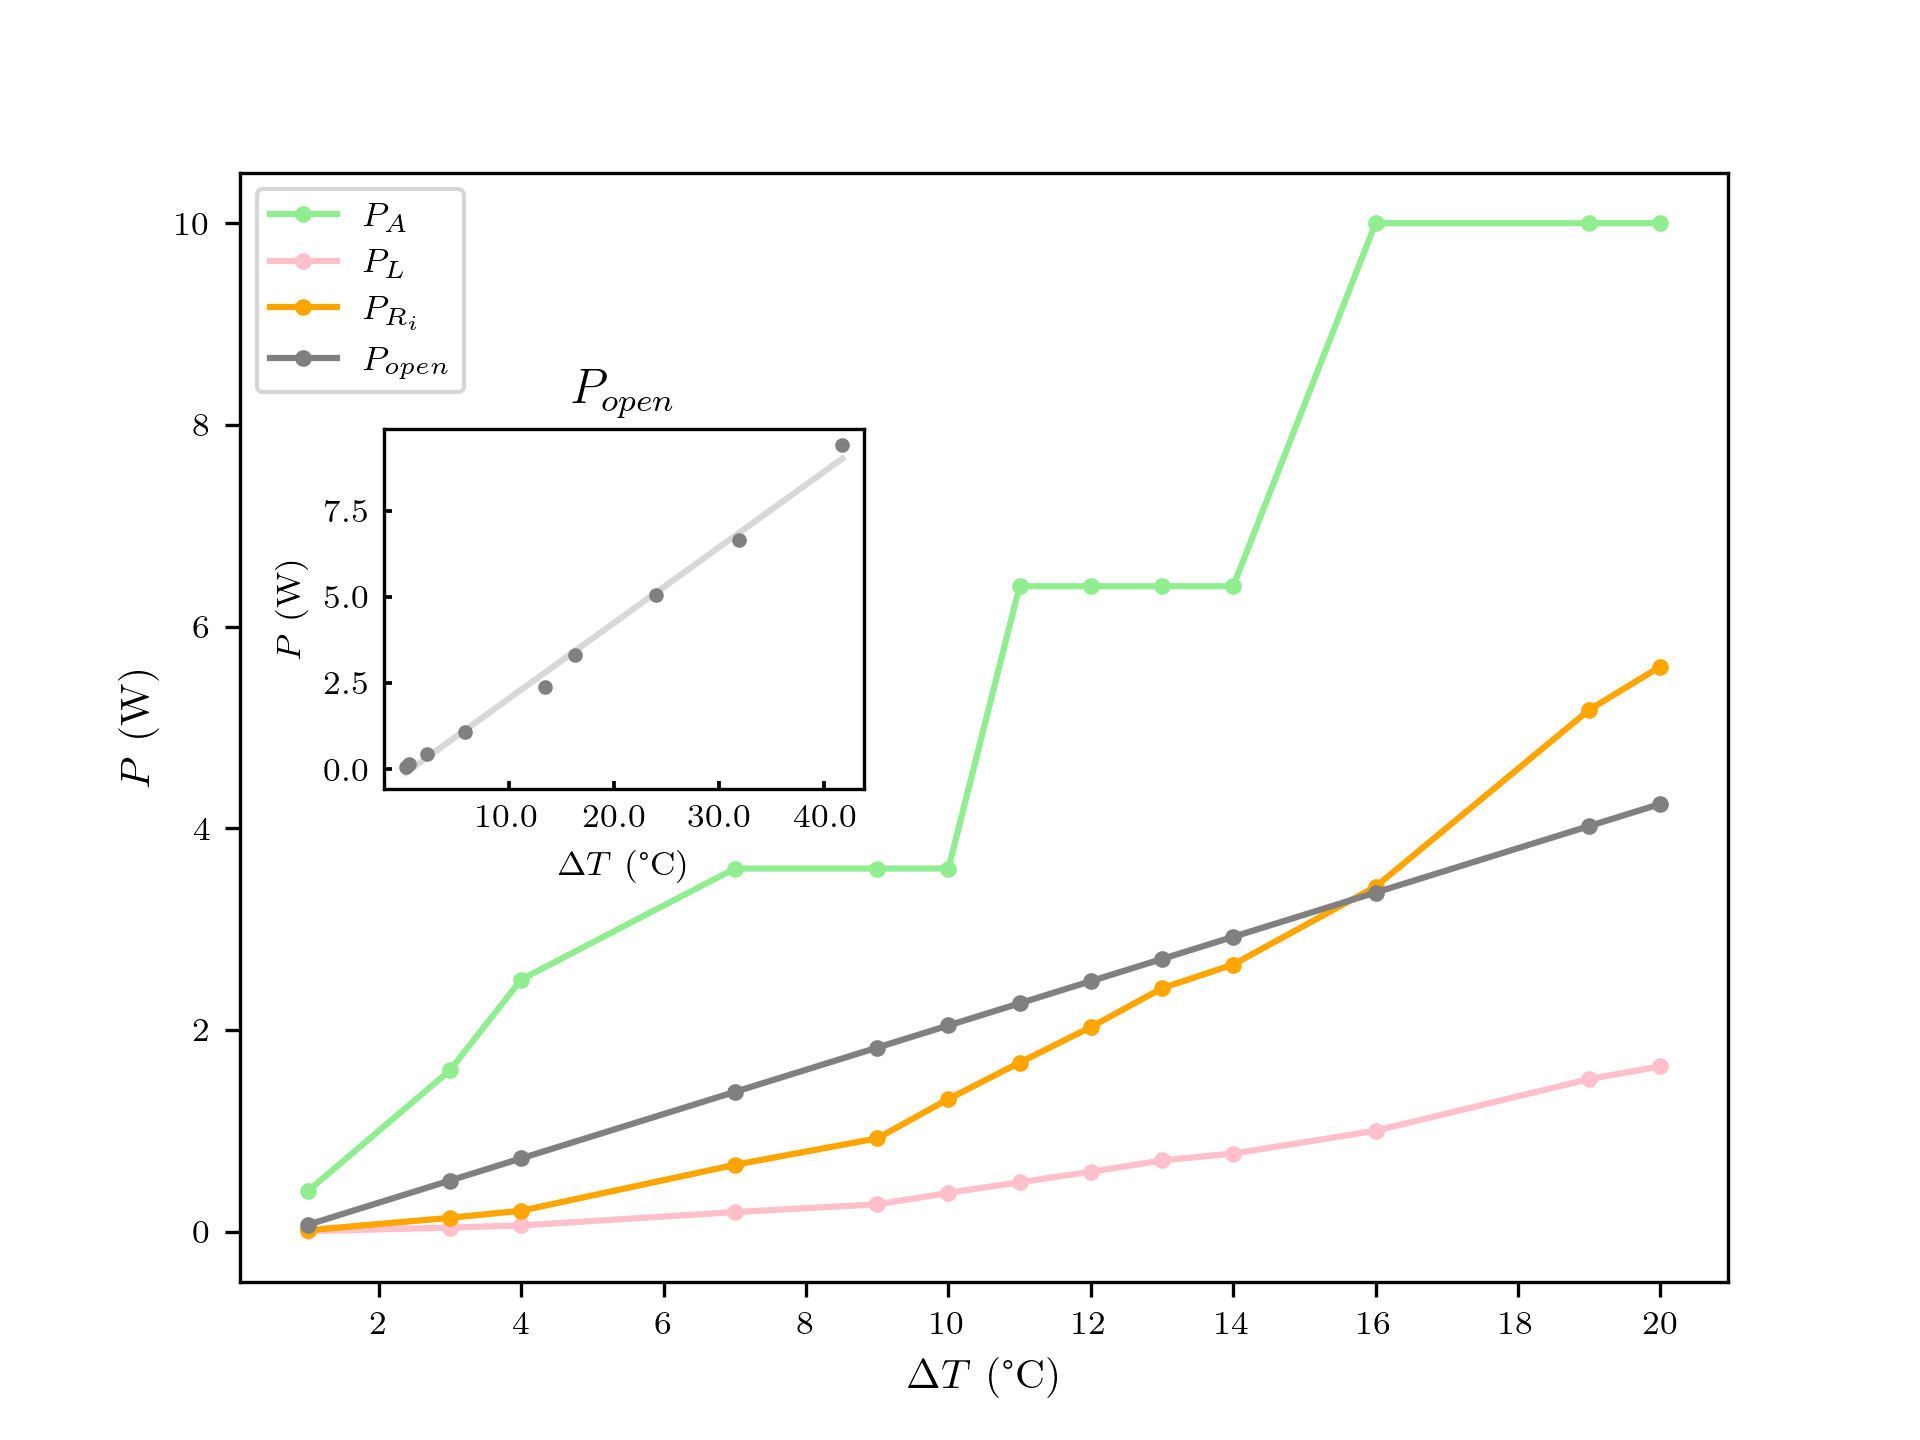
\includegraphics[width = 0.8\linewidth]{img/gen_powers.png}
    \caption{Potencias medidas para el módulo térmico usado como generador térmico. Los datos de $P_{open}$ se midieron en un rango distinto de temperatura y con una escala más fina (décimas de grado).}
    \label{fig:gen_powers}
\end{figure}

Ahora, calculando las eficiencias (nominal, de carnot y corregidas) se obtienen lo mostrado en la figura \ref{fig:etas}. Con esto se tienen más criterios para juzgar los datos. Se puede argumentar que los datos obtenidos para la potencia disipiada por la resistencia interna $P_Ri$ están siendo sobre estimados, pues los valores obtenidos para $\eta^{\prime\prime}$ son mucho mayores a la eficiencia de Carnot, incluso se obtiene valores mayores a 1, por lo que en este caso, esta medición no se considera físicamente correcta.

% etas

\begin{figure}[ht]
    \centering
    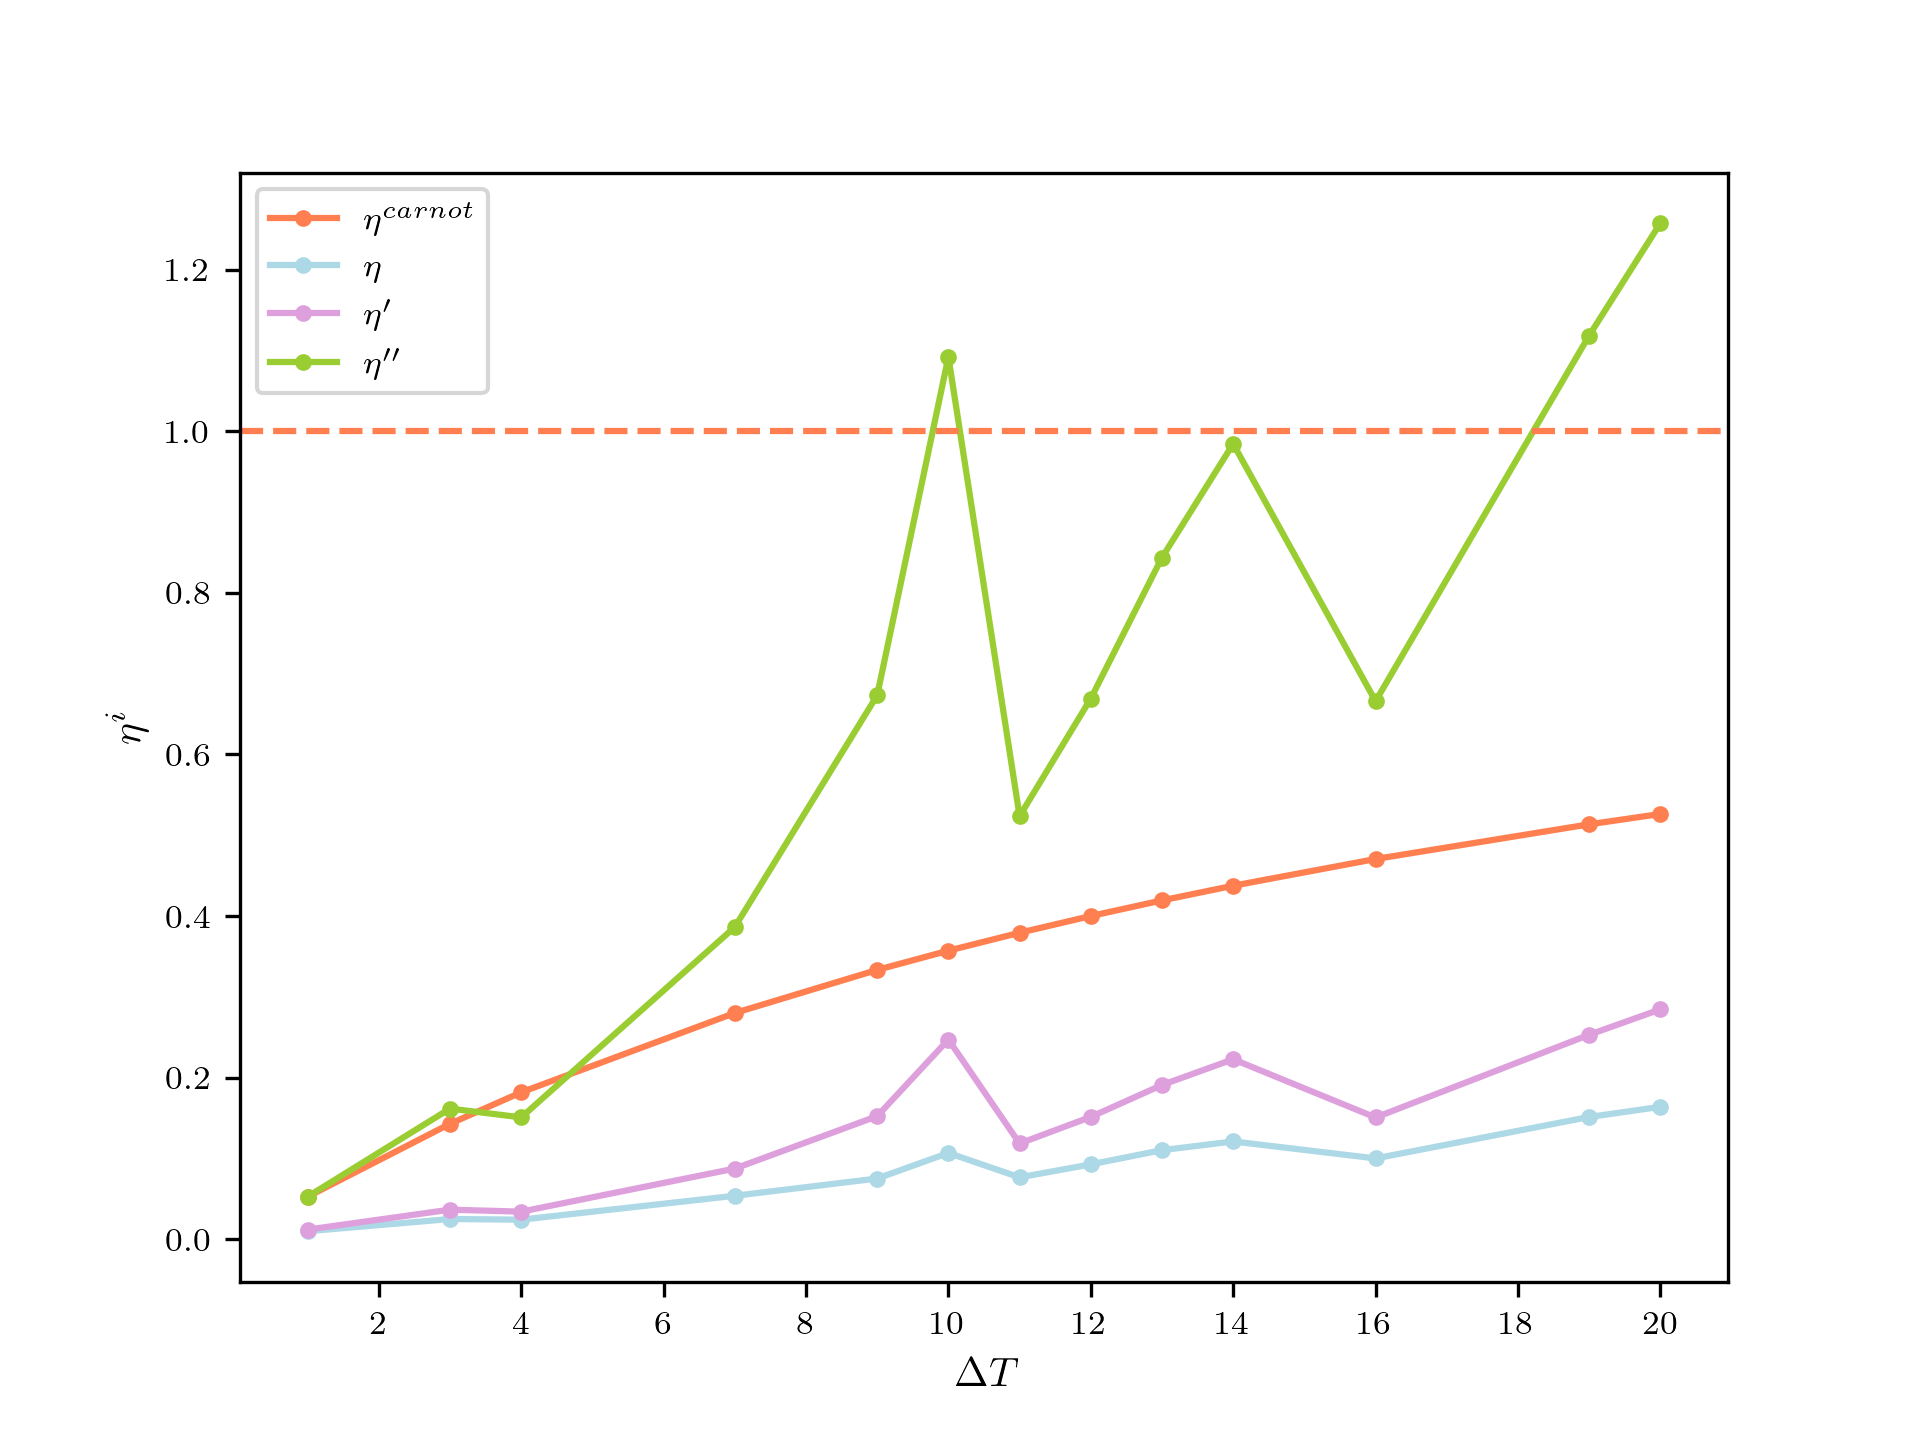
\includegraphics[width = 0.8\linewidth]{img/gen_etas.png}
    \caption{Comparación de las diferentes eficiencias calculadas como función de la diferencia de temperatura}
    \label{fig:etas}
\end{figure}

\subsection{Refrigerador}

\begin{figure}[ht]
    \centering
    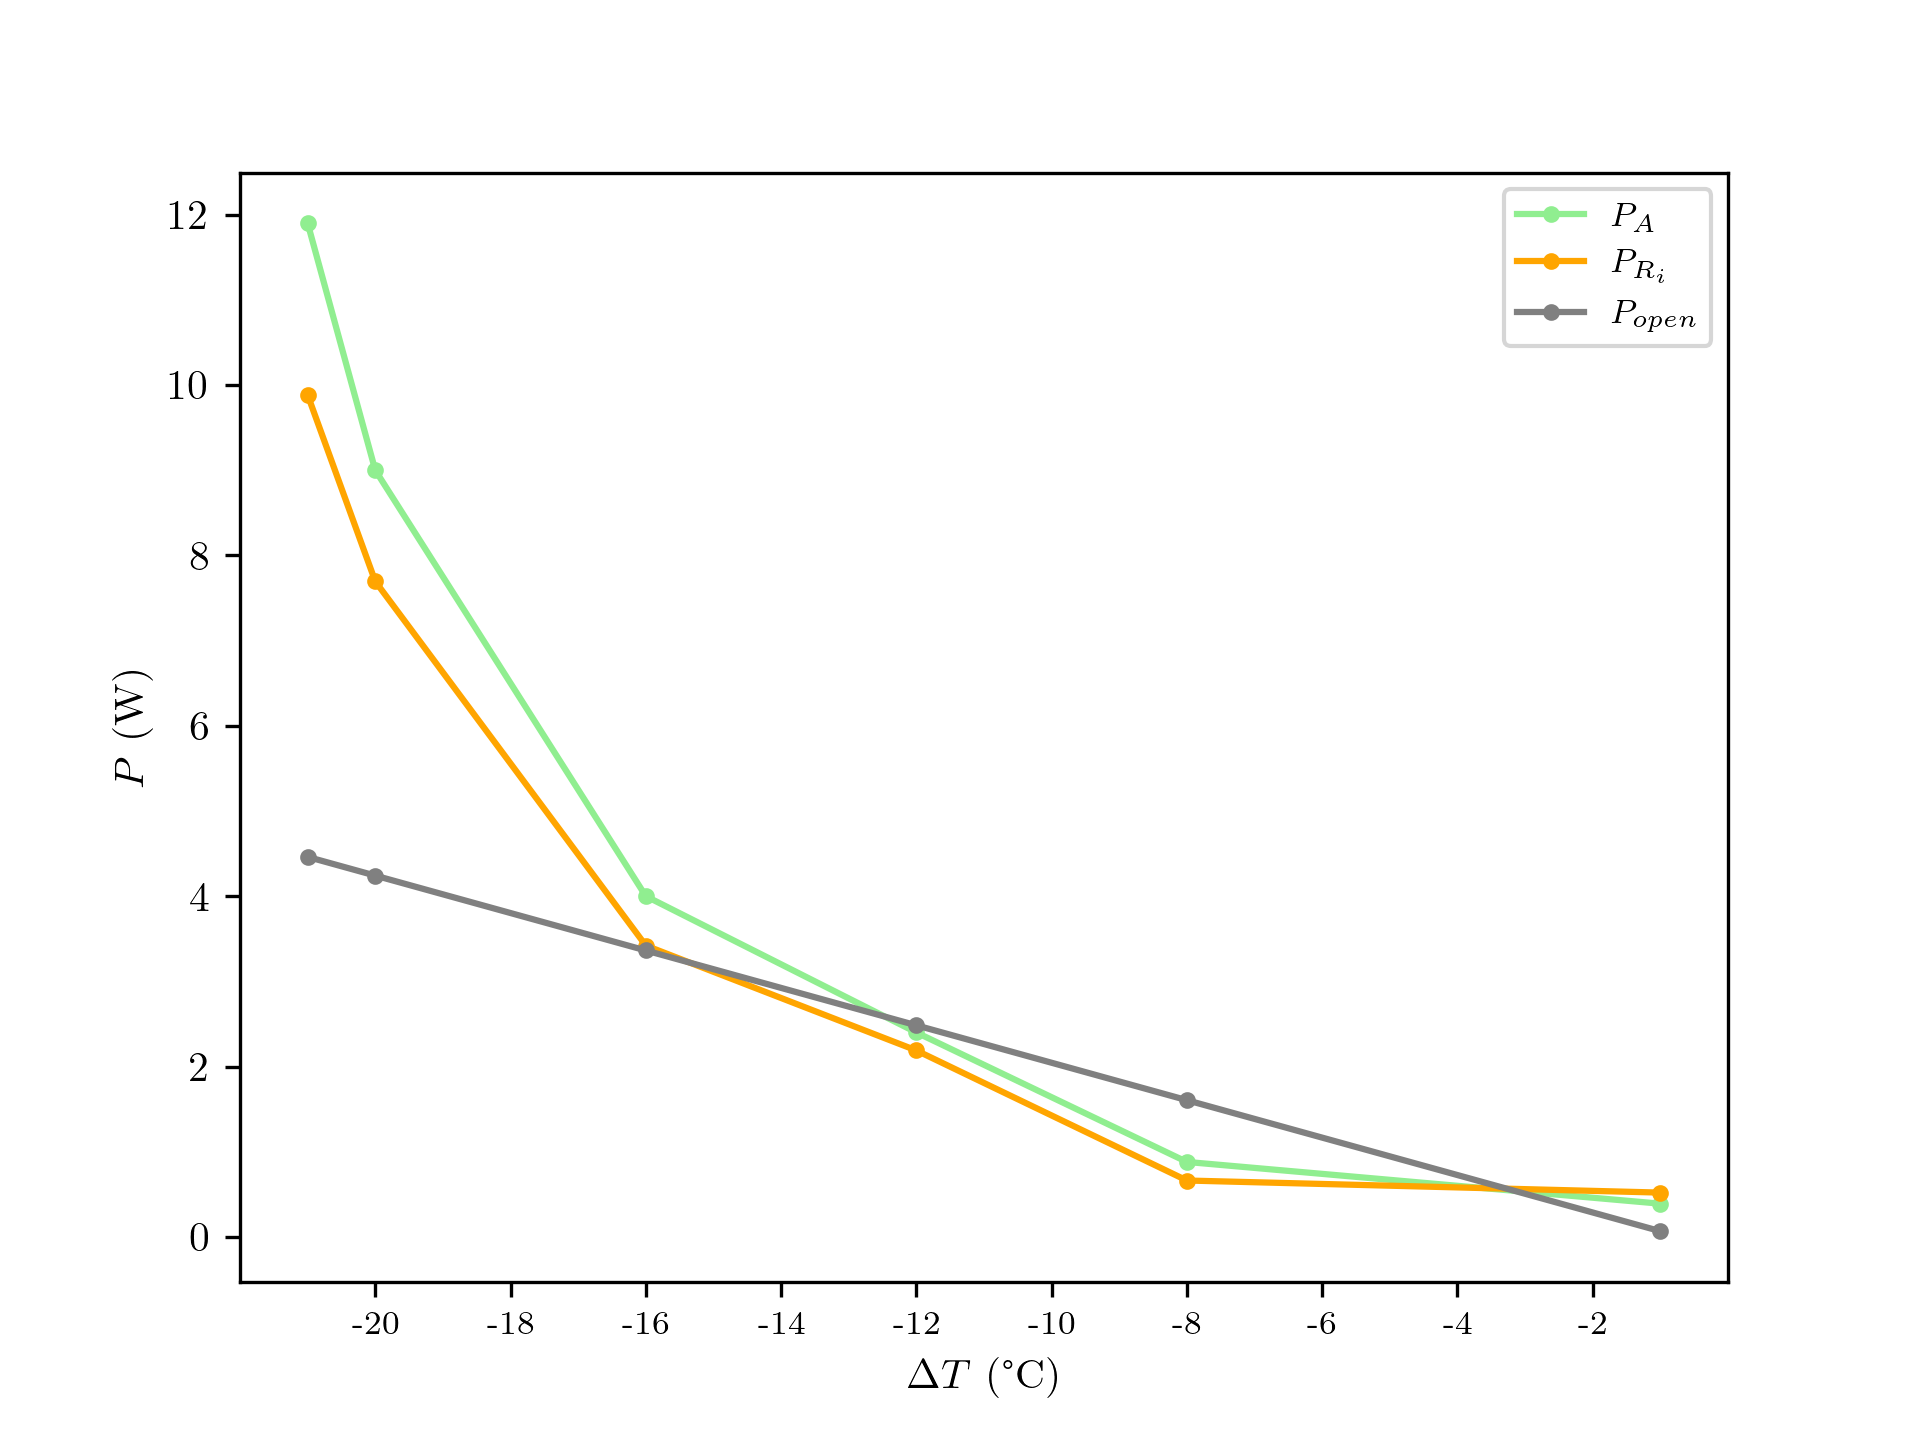
\includegraphics[width = 0.8\linewidth]{img/refri_powers.png}
    \caption{Potencias medidas para el módulo térmico usado como refrigerador. Se usa la misma recta de $P_{open}$ usada en el montaje anterior.}
    \label{fig:refri_powers}
\end{figure}

\begin{figure}[ht]
    \centering
    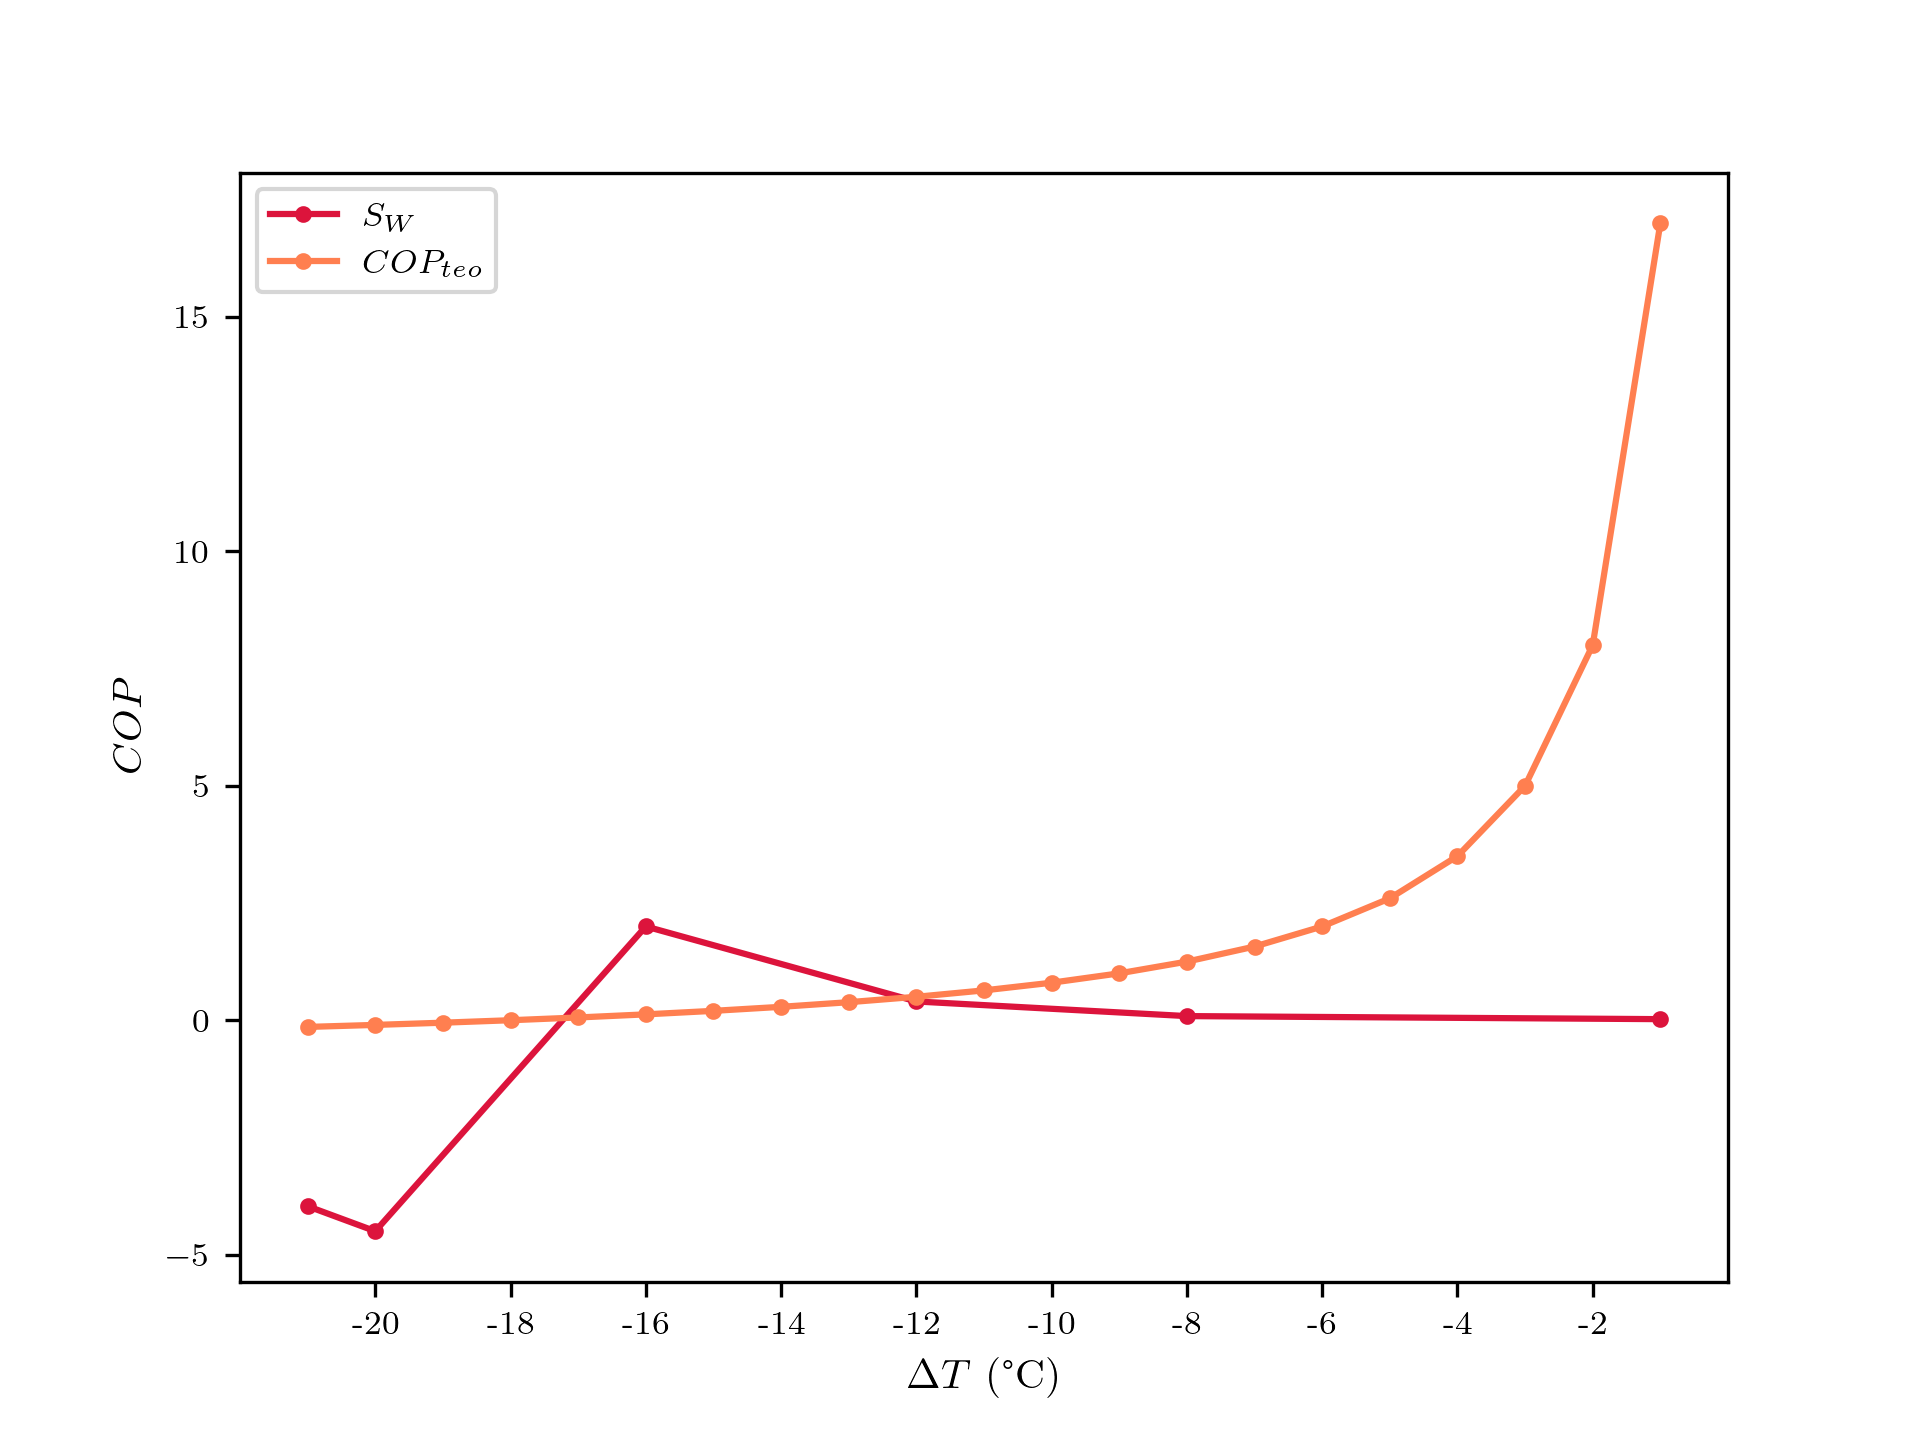
\includegraphics[width = 0.8\linewidth]{img/refri_cops.png}
    \caption{Comparación de los coeficientes de rendimiento.}
    \label{fig:refri_cops}
\end{figure}


\section{Conclusiones}

%\end{multicols}
\printbibliography
\end{document}